\chapter{Architetture Moderne}
Le prestazioni di un programma parallelo dipendono dall’architettura hardware e lo stesso codice può avere prestazioni molto diverse su architetture diverse. Ciò dipende dal fatto che l'architettura determina:
\begin{itemize}
    \item Costi di accesso alla memoria.
    \item Disponibilità di parallelismo.
    \item Costo della computazionale e sincronizzazione.
\end{itemize}
Ignorare questi dettagli potrebbe comportare scelte inefficienti. 
Come già detto, il modello Von Neumann è piuttosto limitante rispetto a quella che è la realtà:
\begin{figure}[H]
    \centering
    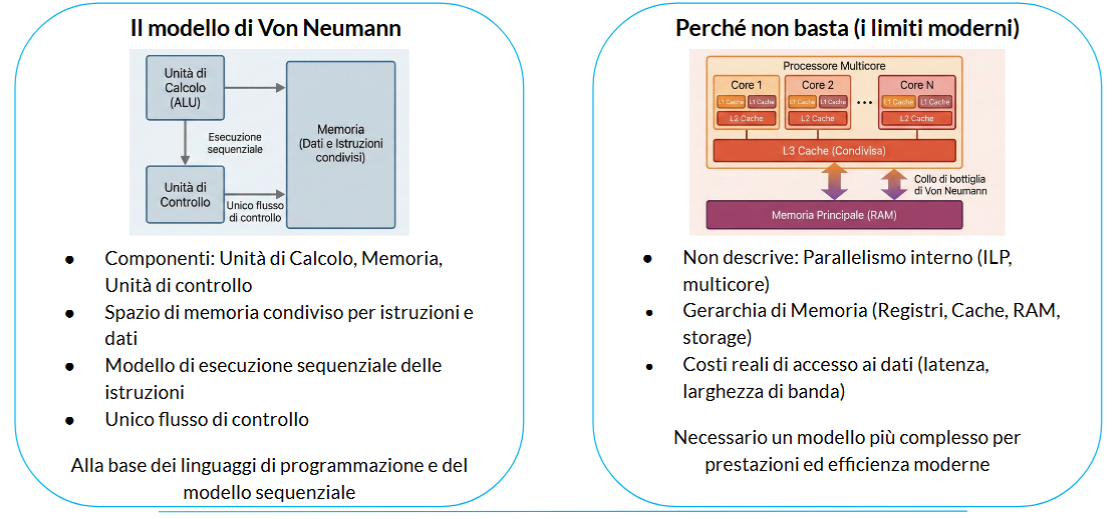
\includegraphics[width=0.85\linewidth]{Images/cap_1/modelli_vs_real.png}
\end{figure}
Infatti, la struttura di un core moderno è molto diversa rispetto a quella ideata da Von Neumann poiché troviamo:
\begin{itemize}
    \item Unita di \textbf{Fetch/Decode}.
    \item \textbf{Pipeline} di esecuzione.
    \item \textbf{Unità di esecuzione} ALU, FPU e unità vettoriali.
    \item \textbf{Registri e Cache di primo livello}
\end{itemize}
\section{Memory Wall}
Il problema principale che dovremo risolvere è quello del \textbf{Memory Wall} per cui il calcolo della \textbf{CPU sia diventato molto più veloce rispetto alla velocità di accesso alla memoria principale} risultando così in sprechi di tempo dovuti al fatto che è necessario attendere l'accesso alla memoria. 
Per cercare di risolvere questo problema, utilizziamo due principi fondamentali:
\begin{itemize}
    \item \textbf{Località temporale}: dati usati di recente vengono spesso riutilizzati.
    \item \textbf{Località spaziale}: dati vicini in memoria vengono utilizzati insieme.
\end{itemize}
Le architetture moderne sfruttano già i principi di località attraverso \textbf{cache, prefetching e gerarchia di memoria}.
\subsection{Gerarchia di Memoria}
I sistemi moderni usano una gerarchia di memoria a più livelli che segue, tipicamente, il seguente schema:
\begin{figure}[H]
    \centering
    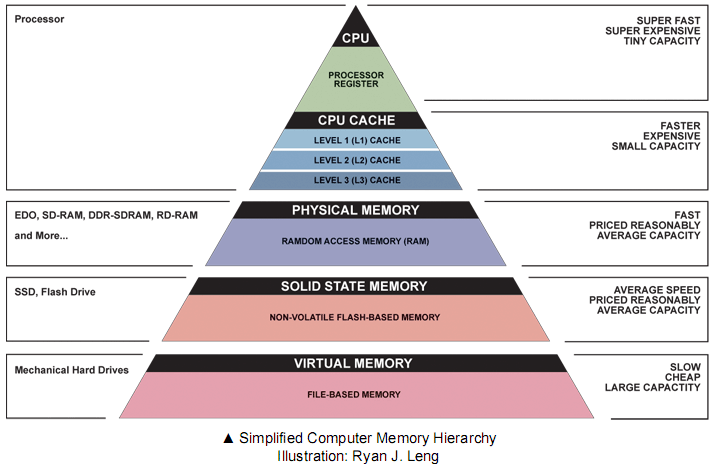
\includegraphics[width=0.85\linewidth]{Images/cap_1/gerarchia_di_memoria.png}
\end{figure}
Ogni livello si differenzia dal precedente in termini di latenza, banda e capacità. Generalmente, minore è la capacità, minore sarà la latenza d'accesso.

Le memorie cache sono memorie molto veloci che memorizzano copie di dati presenti in memoria principale (seguendo il principio di località temporale) e i dati vengono trasferiti tra memoria e cache in \textbf{blocchi} (seguendo il principio di località spaziale).
Abbiamo un \textbf{cache hit} quando il dato è presente in cache, mentre parliamo di \textbf{cache miss} quando il dato non è presente. A causa del costo elevato di accesso in memoria centrale, i cache miss hanno un costo estremamente elevato.
\subsection{Prefetching}
Il \textbf{prefetching} è un meccanismo che anticipa il caricamento dei dati e può essere effettuato tramite \textbf{hardware} o \textbf{software}. Questo può essere parecchio efficace quando abbiamo accessi ai dati regolari con pattern prevedibili ma svantaggio in caso di accessi indiretti o irregolari. Possiamo vedere, ad esempio, i seguenti due snippet di codice:
\begin{figure}[H]
    \centering
    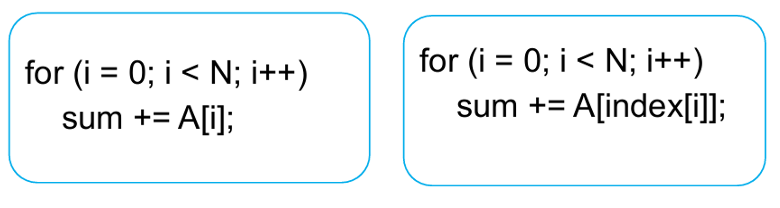
\includegraphics[width=0.6\linewidth]{Images/cap_1/accesso_indiretto.png}
\end{figure}
Quello che vediamo nel secondo caso è che prima di accedere all'indice di A, abbiamo bisogno di accedere a un ulteriore indirizzo di memoria prima. Ciò rallenta chiaramente le prestazioni rispetto al primo caso.
\section{Parallelismo Interno al Processore}
Per aumentare il throughput senza aumentare la frequenza di clock, si sfruttano diverse tecniche di parallelismo.
\subsection{Pipelining}
La \textbf{pipeline} suddivide l’esecuzione di un’istruzione in più stadi:
\begin{itemize}
    \item \textbf{Fetch}: prelevamento dell'istruzione.
    \item \textbf{Decode}: decodifica dell'istruzione.
    \item \textbf{Execute}: accesso ai registri ed esecuzione.
    \item \textbf{Memory Access}: accesso in memoria.
    \item \textbf{Write-back}: scrittura risultato sui registri.
\end{itemize}
Più istruzioni possono essere in esecuzione contemporaneamente in stadi diversi ciò con l’obiettivo di aumentare il throughput. Ci teniamo a sottolineare che il sistema di pipeline non migliora la latenza del sistema poiché questa è una caratteristica intrinseca della gestione della memoria del sistema.
Vedremo più avanti come questo sistema di pipeline in realtà complichi il nostro sistema a causa di possibili stalli dovuti alle dipendenze tra istruzioni o anche a causa di errate guess nel possibile if che verrà eseguito.
\subsection{Instruction-Level Parallelism (ILP)}
L'\textbf{Instruction-Level Parallelism (ILP)} è il parallelismo tra istruzioni indipendenti. Un processore moderno sfrutta l'ILP potendo eseguire più istruzioni nello stesso ciclo di clock e riordinandole dinamicamente (out-of-order execution).
Questo meccanismo è sfruttato tramite:
\begin{itemize}
    \item \textbf{Pipeline multiple}
    \item \textbf{Unità di esecuzione multiple}
\end{itemize}
Il grado di ILP, sebbene sia una tecnica trasparente al programmatore, presenta limiti intrinseci dettati da: dipendenze tra le istruzioni, accessi alla memoria e struttura stessa del codice.
\subsection{SIMD: Parallelismo Vettoriale}
Il \textbf{SIMD (Single Instruction, Multiple Data)} rappresenta un set di istruzione che permette l'applicazione della stessa operazione a più dati contemporaneamente. Le CPU moderne implementano questo paradigma includendo unità vettoriali dotate di registri di grande ampiezza.
La vettorizzazione del codice può essere:
\begin{itemize}
    \item \textbf{Automatica}: a carico del compilatore.
    \item \textbf{Esplicita}: a carico del programmatore. Sebbene molto efficace, la velocità ottenibile dal SIMD dipende strettamente dalla regolarità degli accessi in memoria e dall'assenza di dipendenze tra le iterazioni.
\end{itemize}
\subsection{SMT: Simultaneous Multithreading}
Il \textbf{SMT (Simultaneous Multithreading)} permette a un singolo core di eseguire più thread hardware contemporaneamente. In questo scenario, i thread condividono pipeline, unità di esecuzione e cache.
Lo SMT mira a:
\begin{itemize}
    \item Migliorare l'utilizzo delle risorse del core.
    \item Nascondere le latenze (come gli accessi in memoria).
\end{itemize}
È fondamentale notare che lo SMT non raddoppia le prestazioni, poiché i thread competono per le medesime risorse. La sua reale efficacia dipende dal tipo di carico di lavoro e dal comportamento della memoria. Sarebbe bene che thread hardware che condividono lo stesso core, utilizzino gli stessi dati così da evitare da poter sfruttare al meglio la cache L1 che condividono. Se non facessero a questo modo, si rischierebbe che i buttano fuori i datti dalla memoria a vicenda.
\section{Sistemi Multicore e Modelli di Accesso alla Memoria}
I \textbf{processori multicore} integrano più core di calcolo sullo stesso chip. Questa architettura rappresenta la principale risposta hardware alla fine dello scaling di Dennard e all'impossibilità fisica di continuare ad aumentare la frequenza di clock.
In un sistema multicore:
\begin{itemize}
    \item \textbf{Risorse private}: ogni core dispone di proprie pipeline, unità di esecuzione e cache (tipicamente L1 e L2).
    \item \textbf{Risorse condivise}: la cache di ultimo livello (L3) e la memoria principale sono condivise tra i core.
\end{itemize}
\begin{figure}[H]
    \centering
    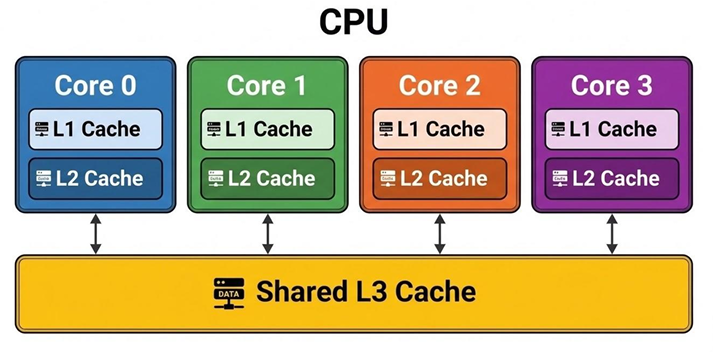
\includegraphics[width=0.6\linewidth]{Images/cap_1/multicore.png}
\end{figure}
Le prestazioni finali di un processore multicore dipendono pesantemente dalla capacità del software di sfruttare più core in parallelo e di gestire in modo efficiente la condivisione delle risorse.
\subsection{Il Modello MIMD}
L'architettura \textbf{MIMD (Multiple Instruction, Multiple Data)} prevede che ogni unità di elaborazione esegua un flusso di istruzioni indipendente operando su dati differenti. Questo modello a parallelismo coarse-grained offre elevata flessibilità, è adatto a problemi eterogenei e rappresenta la base dei sistemi moderni.
\subsection{SMP vs NUMA}
Nei sistemi \textbf{SMP (Symmetric Multiprocessing)}, più processori condividono la stessa memoria fisica e lo stesso spazio di indirizzamento.
Si basano su un modello UMA (Uniform Memory Access), dove l'accesso alle risorse è paritario per tutti i processori ed equivalenti per il sistema operativo.
\begin{itemize}
    \item \textbf{Vantaggi}: modello concettualmente semplice, comunicazione veloce intra-nodo e forte supporto da parte di OS e runtime.
    \item \textbf{Svantaggi}: scalabilità limitata (difficile andare oltre poche decine di core) a causa della contesa sul bus di memoria e del traffico hardware dovuto a protocolli necessari a mantenere la coerenza della cache.
\end{itemize}
Per superare i limiti di scalabilità dell'SMP, si utilizza \textbf{l'architettura NUMA (Non-Uniform Memory Access)}, in cui la memoria è fisicamente distribuita.
Ogni gruppo di core possiede una memoria locale (con accesso più veloce), ma può accedere alla memoria remota (con accesso più lento).

I sistemi moderni sono spesso ccNUMA (cache-coherent NUMA): l'hardware mantiene la coerenza delle cache tra i vari nodi NUMA, offrendo al programmatore l'illusione di una memoria condivisa. Le prestazioni reali dipendono fortemente dalla località NUMA dei dati e dei thread.
\section{Sistemi a Memoria Condivisa e Distribuita}
In base al paradigma di accesso alla memoria, possiamo dividere i sistemi in due macro-categorie:
\begin{itemize}
    \item \textbf{Sistemi a memoria condivisa}: Tutti i thread vedono lo stesso spazio di indirizzamento e comunicano implicitamente tra loro leggendo e scrivendo gli stessi dati. Il parallelismo è espresso tramite thread. La programmazione è generalmente più semplice, ma presenta svantaggi legati alla competizione per le risorse, la necessità di sincronizzazione e i costi di memoria non uniformi introdotti dalle architetture NUMA.
    \item \textbf{Sistemi a memoria distribuita}: Ogni processo dispone di una memoria privata e non esiste alcuno spazio di indirizzamento globale. La comunicazione tra processi avviene obbligatoriamente tramite lo scambio esplicito di messaggi. Questo approccio garantisce un'elevata scalabilità e rimuove la contesa diretta sulla memoria, al prezzo di una programmazione più complessa e di un costo esplicito (latenza) per ogni comunicazione.
\end{itemize}
\subsection{Sistemi Ibridi e HPC}
I sistemi ibridi costituiscono l'architettura standard per i moderni sistemi HPC:
\begin{itemize}
    \item Sono composti da nodi multicore che operano internamente a memoria condivisa.
    \item Questi nodi sono poi collegati tra loro formando un cluster a memoria distribuita.
\end{itemize}
Di conseguenza, la gestione del parallelismo avviene su due livelli distinti e complementari:
\begin{itemize}
    \item All'interno del singolo nodo (Intra-nodo): il parallelismo viene espresso tramite thread che accedono alla memoria condivisa locale (spessore regolato da architettura NUMA).
    \item Tra nodi diversi (Inter-nodo): il parallelismo è gestito tramite processi separati, e lo scambio di dati richiede una comunicazione esplicita (come l'invio di messaggi via rete).
\end{itemize}
\subsection{Reti e Acceleratori}
Nei sistemi HPC i nodi sono collegati tramite \textbf{reti ad alte prestazioni} e questa influenza la \textbf{latenza} della comunicazione, la \textbf{banda} disponibile e la \textbf{scalabilità} delle applicazioni. È anche possibile fare uso di \textbf{acceleratori} come dispositivi specializzati per il calcolo parallelo come la \textbf{GPU}.
\section{Modelli di Analisi: Il Roofline Model}
Il \textbf{Roofline model} è un modello prestazionale semplificato. Questo descrive il limite massimo di prestazioni di un'applicazione che è solitamente limitato a causa di capacità di calcolo o dalla banda di memoria. Questo modello mette in relazione \textbf{intensità computazionale} e \textbf{prestazioni ottenibili}. 
Esistono due tipi di sistemi:
\begin{itemize}
    \item \textbf{memory bound}.
    \item \textbf{compute bound}.
\end{itemize}
E questo modello ci aiuta a capire dove intervenire per ottimizzare al variare di memoria messa a disposizione o potenza computazionale messa a disposizione.

